\def\duedate{10/24/22}
\def\HWnum{3}
% Document setup
\documentclass[12pt]{article}
\usepackage[margin=1in]{geometry}
\usepackage{fancyhdr}
\usepackage{lastpage}

\pagestyle{fancy}
\lhead{Richard Whitehill}
\chead{PHYS 675 -- HW \HWnum}
\rhead{\duedate}
\cfoot{\thepage \hspace{1pt} of \pageref{LastPage}}

% Encoding
\usepackage[utf8]{inputenc}
\usepackage[T1]{fontenc}

% Math/Physics Packages
\usepackage{amsmath}
\usepackage{mathtools}
\usepackage[arrowdel]{physics}
\usepackage{siunitx}

\AtBeginDocument{\RenewCommandCopy\qty\SI}

% Reference Style
\usepackage{hyperref}
\hypersetup{
    colorlinks=true,
    linkcolor=blue,
    filecolor=magenta,
    urlcolor=cyan,
    citecolor=green
}

\newcommand{\eref}[1]{Eq.~(\ref{eq:#1})}
\newcommand{\erefs}[2]{Eqs.~(\ref{eq:#1})--(\ref{eq:#2})}

\newcommand{\fref}[1]{Fig.~\ref{fig:#1}}
\newcommand{\frefs}[2]{Figs.~\ref{fig:#1}--\ref{fig:#2}}

\newcommand{\tref}[1]{Table~\ref{tab:#1}}
\newcommand{\trefs}[2]{Tables~\ref{tab:#1}-\ref{tab:#2}}

% Figures and Tables 
\usepackage{graphicx}
\usepackage{float}
\usepackage{booktabs}

\newcommand{\bef}{\begin{figure}[h!]\begin{center}}
\newcommand{\eef}{\end{center}\end{figure}}

\newcommand{\bet}{\begin{table}[h!]\begin{center}}
\newcommand{\eet}{\end{center}\end{table}}

% tikz
\usepackage{tikz}
\usetikzlibrary{calc}
\usetikzlibrary{decorations.pathmorphing}
\usetikzlibrary{decorations.markings}
\usetikzlibrary{arrows.meta}
\usetikzlibrary{positioning}

% tcolorbox
\usepackage[most]{tcolorbox}
\usepackage{xcolor}
\usepackage{xifthen}
\usepackage{parskip}

\newcommand*{\eqbox}{\tcboxmath[
    enhanced,
    colback=black!10!white,
    colframe=black,
    sharp corners,
    size=fbox,
    boxsep=8pt,
    boxrule=1pt
]}

% Miscellaneous Definitions/Settings
\newcommand{\prob}[2]{\textbf{#1)} #2}

\setlength{\parskip}{\baselineskip}
\setlength{\parindent}{0pt}
\setlength{\headheight}{14.49998pt}
\addtolength{\topmargin}{-2.49998pt}


\begin{document}
    
\prob{1}{}

a) What are the possible $J^{PC}$ (total angular momentum, parity, and charge quantum numbers) values for mesons made up of a quark and an antiquark of the same flavor?
Enumerate all the possibilities through $J = 4$.

The total angular momentum $J = L + S$, where $L$ is the orbital angular momentum and $S$ is the spin angular momentum. 
Since the meson system ($q\overline{q}$) is composed of 2 fermions, it must be a boson, meaning it can only be spin-0 or spin-1.
The total angular momentum for a given $s,\ell$ values for spin and orbital angular momentum $j \in \{ |s - \ell|, \ldots, s + \ell - 1, s + \ell \} $.
The parity quantum number is multiplicative, with $P(\overline{q}) = - P(q)$ and $|P(q)| = 1$.
Thus, $P(q\overline{q}) = -[P(q)]^2(-1)^{\ell} = (-1)^{\ell + 1}$.
Additionally, the charge quantum number takes on the value $(-1)^{\ell + s}$ for a system consiting of a particle-antiparticle pair.

\begin{table}[H]
\begin{center}
\begin{tabular}{ccccc}
    S & L & J & P & C\\
    \hline
    0 & 0 & 0 & - & + \\
    1 & 0 & 1 & - & - \\
    0 & 1 & 1 & + & - \\
    1 & 1 & $\{ 0,1,2 \} $ & + & + \\
    0 & 2 & 2 & - & + \\
    1 & 2 & $\{ 1,2,3 \} $ & - & - \\
    0 & 3 & 3 & + & - \\
    1 & 3 & $\{ 2,3,4 \} $ & + & + \\
    0 & 4 & 4 & - & +
\end{tabular}
\end{center}
\caption{Table of possible $J$ and $P$ values for unflavored mesons given combinations of $S$ and $L$ values.}
\label{tab:JPC-values}
\end{table}

These combinations give us the following set of possible $J^{PC}$ values:
\begin{align}
    \label{eq:JPC}
    J^{PC} &\in \{ 0^{-+}, 1^{--}, 1^{+-}, 0^{++}, 1^{++}, 2^{++}, 2^{-+}, 2^{--}, 3^{--}, 3^{+-}, 3^{++}, 4^{++}, 4^{-+} \}
.\end{align}

b) Which of these values can be found for mesons in the PDG listings? 

The PDG lists the following values of $J^{PC}$ in the light unflavored meson section, which correspond with the list in \eref{JPC}:
\begin{align}
    \label{eq:JPC-PDG}
    \{ 0^{-+}, 0^{++}, 1^{--}, 1^{+-}, 1^{++}, 2^{++}, 1^{--}, 2^{-+}, 3^{--}, 4^{++} \} 
.\end{align}


c) What $J^{PC}$ values are not possible for a quark-antiquark pair?
Can any of them be found in the PDG listings?

The following $J^{PC}$ values are listed in the PDG, which are not listed in \eref{JPC}:
\begin{eqnarray}
    \label{eq:JPC-forbidden}
    \{ 1^{-+} \}  
.\end{eqnarray}
Clearly, this indicates that our model for mesons simply as $q\overline{q}$ pairs is insufficient and incorrect.

d) What $J^{PC}$ values are possible for a meson that decays strongly into $\pi^{+}\pi^{-}$?

The $\pi^{\pm}$ have $J = 0$ and $P = -1$ separately.
As a system $P = (-1)^{\ell}$, and $J = 0$, assuming sufficiently low energy.
In any strong decay, parity and spin is conserved so it follows that the possible values of $J^{PC} = 0^{+\pm}$.

e) What $J^{PC}$ values are possible for a meson that decays strongly into $\pi^{0}\pi^{0}$?
What are the possible isospin values?

We know $J^{PC} = 0^{-+}$ for the $\pi^{0}$.
As a system $P = -1$ and $C = -1$, so we need $J = 0$ and $J^{PC} = 0^{--}$.

From isospin considerations $\pi^{0} = \ket{1,0}$, and using the Clebsch-Gordan coefficients, we can write
\begin{eqnarray}
    \label{eq:isospin-CG}
    \ket{1,0}\ket{1,0} = \sqrt{\frac{2}{3}}\ket{2,0} - \sqrt{\frac{1}{3}}\ket{0,0}
,\end{eqnarray}
so the initial meson could have isospin $0$ or $2$.

f) If you discovered a spin-0 meson that decays strongly into $\rho^{0}\pi^{0}$, why would you want to rush this result off for immediate publication?

We strongly believe that spin is a conserved quantity (it is essentially a law) in a strong decay or scattering process.
The initial state has spin-0 (as given), but the final state has spin-1 ($s_{\rho} = 1$ and $s_{\pi} = 0$).
This would be a monumental finding if true since it would be the first observed instance of spin conservation being violated in strong interactions.

\prob{2}{
Show that the $\eta(548)$ meson cannot decay into 2 pions by either the strong or electromagnetic interactions and that it cannot decay into 3 pions by the strong interactions.
}

The $\eta$ meson has $J^{PC} = 0^{-+}$ and is (iso)spin-0, where the pions have $J = 0$ and $P = -1$ ($C = +1$ for the $\pi^{0}$).
For a two pion system, we have $P = 1$, so it is clear that an $\eta$ decay into two pions is impossible electromagnetically and strongly, which both conserve parity.
Notice that for a three pion system, $G = -1$ but $G = +1$ for the $\eta$ meson, and since G-parity is conserved in a strong interaction, the $\eta$ cannot decay via the strong interaction into $3$ pions.



\prob{3}{
Write an equation relating the cross sections for these four reactions:
\begin{eqnarray}
    \label{eq:reactions}
    \begin{cases}
        (a)~\overline{K}^{0}p \rightarrow \Sigma^{0}\pi^{+} \\
        (b)~\overline{K}^{0}n \rightarrow \Sigma^{+}\pi^{-} \\
        (c)~\overline{K}^{0}n \rightarrow \Sigma^{0}\pi^{0} \\
        (d)~\overline{K}^{0}n \rightarrow \Sigma^{-}\pi^{+}
    \end{cases}
.\end{eqnarray}
}

The proton and neutron isospin wavefunctions are $\ket{1/2,1/2}$ and $\ket{1/2,-1/2}$, respectively, and the $\overline{K}^{0} = s\overline{d}$ has isospin wavefunction $\ket{1/2,1/2}$.
Let the amplitudes for the reactions above be labeled $\mathcal{M}_{a,b,c,d}$, corresponding to their label above and the amplitudes resulting in isospin final states $I = 1,0$ be $\mathcal{M}_{1,0}$, respectively.

Additionally, the $\Sigma^{+}$, $\Sigma^{0}$, and $\Sigma^{-}$ have isospin wavefunctions $\ket{1,1}$, $\ket{1,0}$, $\ket{1,-1}$.
Thus, for the $\overline{K}^{0}p$ collision
\begin{align}
    \label{eq:rxn1}
    \ket{1/2,1/2}\ket{1/2,1/2} &= \ket{1,1} \\
    \ket{1,0}\ket{1,1} &= \frac{1}{\sqrt{2}}\big[ \ket{2,1} - \ket{1,1} \big]
,\end{align}
while for the $\overline{K}^{0}n$ collisions
\begin{align}
    \label{eq:rxn2-4}
    \ket{1/2,1/2}\ket{1/2,-1/2} &= \frac{1}{\sqrt{2}}\big[ \ket{1,0} + \ket{0,0} \big] \\
    \ket{1,1}\ket{1,-1} &= \Big[ \frac{1}{\sqrt{6}}\ket{2,0} + \frac{1}{\sqrt{2}}\ket{1,0} + \frac{1}{\sqrt{3}}\ket{0,0} \Big] \\
    \ket{1,0}\ket{1,0} &= \Big[ \sqrt{\frac{2}{3}}\ket{2,0} - \frac{1}{\sqrt{3}}\ket{0,0} \Big] \\
    \ket{1,-1}\ket{1,1} &= \Big[ \frac{1}{\sqrt{6}}\ket{2,0} - \frac{1}{\sqrt{2}}\ket{1,0} + \frac{1}{\sqrt{3}}\ket{0,0} \Big]
.\end{align}
Hence, 
\begin{align}
    \label{eq:amplitude-relations}
    \mathcal{M}_{a} &= -\frac{1}{\sqrt{2}}\mathcal{M}_{1} \\
    \mathcal{M}_{b} &= \frac{1}{2}\mathcal{M}_{1} + \frac{1}{\sqrt{6}}\mathcal{M}_{0} \\
    \mathcal{M}_{c} &= -\frac{1}{\sqrt{6}}\mathcal{M}_{0} \\
    \mathcal{M}_{d} &= -\frac{1}{2}\mathcal{M}_{1} + \frac{1}{\sqrt{6}}\mathcal{M}_{0}
.\end{align}
The cross sections are then
\begin{align}
    \label{eq:cs-from-amps}
    \sigma_{a} &= \frac{1}{2}|\mathcal{M}_{1}|^2 \\
    \sigma_{b} &= \frac{1}{2} \Big| \mathcal{M}_{1} + \sqrt{\frac{2}{3}}\mathcal{M}_{0} \Big|^2 \\
    \sigma_{c} &= \frac{1}{6}|\mathcal{M}_{0}|^2 \\
    \sigma_{d} &= \frac{1}{2} \Big| \mathcal{M}_{1} - \sqrt{\frac{2}{3}}\mathcal{M}_{0} \Big|^2
.\end{align}
Now, we can relate the total cross sections for $\overline{K}^{0}p(n)$ scattering
\begin{eqnarray}
    \label{eq:total-cs}
    R = \frac{\sigma_{\rm tot}(\overline{K}^{0}p)}{\sigma_{\rm tot}(\overline{K}^{0}n)} = \frac{\sigma_{a}}{\sigma_{b} + \sigma_{c} + \sigma_{d}} = \frac{|\mathcal{M}_{1}|^2}{|\mathcal{M}_{1}|^2 + 5|\mathcal{M}_{0}|^2/6} = \frac{1}{1 + \frac{5}{6}\Big| \frac{\mathcal{M}_{0}}{\mathcal{M}_{1}} \Big|^2}
.\end{eqnarray}


\prob{4}{
    As an example of the use of isospin in weak decays, consider the decays $\tau^{+} \rightarrow \pi^{+}\pi^{+}\pi^{-}\overline{\nu}_{\tau}$ and $\tau^{+} \rightarrow \pi^{+}\pi^{0}\pi^{0}\overline{\nu}_{\tau}$.
}

a) Draw the diagram for these decays at the quark level (before hadronization) and observe that there is only one possible isospin state.

The base diagram for these decays mediated by a $W$ boson is shown below.
The two processes differ only by the specifics of how hadronization occurs on the legs of the $u$ and $\overline{d}$ quarks.
It is is clear that the state $u\overline{d}$ only has one isospin state since $u$ and $\overline{d}$ are in the isospin state $\ket{1/2,1/2}$.

\begin{figure}[H]
\begin{center}
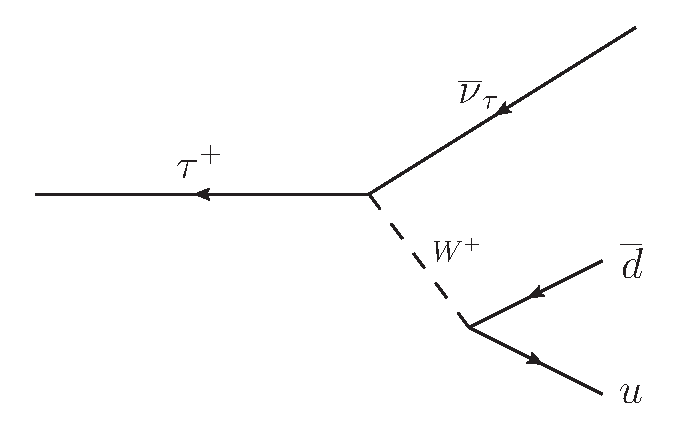
\includegraphics[width=0.6\textwidth]{prob4.eps}
\end{center} 
\end{figure}

b) There is strong evidence that the three pions in these decays come from a $\rho \pi$ intermediate state.
Assuming that, predict the ratio of branching fractions for these two decays.
Compare to data (PDG).

The $\rho^{\pm}$ and $\rho^{0}$ are essentially excited states of the $\pi^{\pm}$ and $\pi^{0}$, respectively, so their isospin wavefunctions are the same.
In either case, we have the isospin wavefunction of the state as
\begin{eqnarray}
    \label{eq:rho-pi}
    \ket{1,1}\ket{1,0} = \frac{1}{\sqrt{2}} \big[ \ket{2,1} + \ket{1,1} \big]
.\end{eqnarray}
Now for the final states, we have
\begin{align}
    \label{eq:final-states}
    \ket{1,1}\ket{1,1}\ket{1,-1} &= \ket{2,2}\ket{1,-1} = \frac{1}{\sqrt{15}}\ket{3,1} + \frac{1}{\sqrt{3}}\ket{2,1} + \sqrt{\frac{3}{5}}\ket{1,1} \\
    \ket{1,1}\ket{1,0}\ket{1,0} &= \frac{1}{\sqrt{2}}\big[ \ket{2,1}\ket{1,0} + \ket{1,1}\ket{1,0} \big] \notag \\
                                &= \frac{2}{\sqrt{15}}\ket{3,1} + \frac{1}{2\sqrt{3}}\ket{2,1} - \frac{1}{2}\sqrt{\frac{3}{5}}\ket{1,1} + \frac{1}{2}\ket{2,1} + \frac{1}{2}\ket{1,1}
.\end{align}
Hence, the branching ratio is
\begin{eqnarray}
    \label{eq:B}
\mathcal{B} = \frac{|\bra{1,1}\bra{1,1}\bra{1,-1} \ket{1,1}\ket{1,0}|^2}{|\bra{1,1}\bra{1,0}\bra{1,0} \ket{1,1}\ket{1,0}|^2} = \frac{4\big| 1/\sqrt{6} + \sqrt{3/10} \big|^2}{\big|(1/\sqrt{6} + 1) + 1/\sqrt{2}(1 - \sqrt{3/5}) \big|^2} \approx 2.3
.\end{eqnarray}

The PDG lists branching ratio into 3 charged pions as 8.99\% and the branching ratio into a charged pion and 2 neutral pions as 9.26\%, so the actual branching ratio is $0.97$.
These answers are not in agreement.
The discrepancy may come from how we wrote the wavefunction since there are a couple indistinguishable bosons in the final state in each decay.

\prob{5}{
The neutral vector mesons all have measurable decays into $e^{+}e^{-}$.
The diagram for this decay is shown below.
Since the quark and antiquark are in a bound state, the calculation of these decay rates depends on the vector meson wave functions and masses.
However, it is reasonable to assume that these are all about the same for the three light neutral vector mesons, the $\rho^{0}$, the $\omega$, and the $\phi$.
Make this assumption and predict the relative partial widths.
}

\begin{center}
    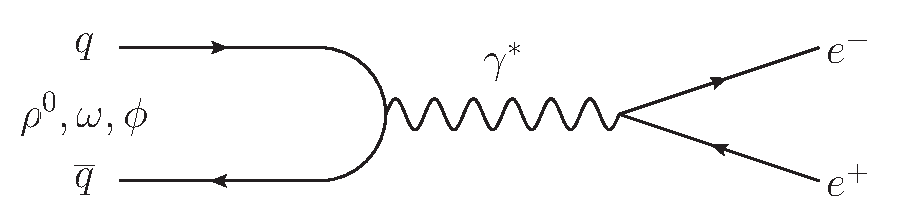
\includegraphics[width=0.6\textwidth]{prob5.eps} 
\end{center}


The quark wavefunctions for the mesons above are as follows:
\begin{align}
    \label{eq:q-wavefuncs}
    \rho^{0} &= \frac{1}{\sqrt{2}}\Big[ u\overline{u} - d\overline{d} \Big] \\
    \omega &= \frac{1}{\sqrt{2}}\Big[ u\overline{u} + d\overline{d} \Big] \\
    \phi &= s\overline{s}
.\end{align}
Note that the primary difference between any $q\overline{q} \rightarrow e^{+}e^{-}$ cross section comes from the charge at the vertex.
Hence,
\begin{align}
    \label{eq:vertex-factors}
    \mathcal{M}_{\rho} &\propto \frac{1}{\sqrt{2}} \Big[ \frac{2}{3} -  \Big( -\frac{1}{3} \Big) \Big] = \frac{1}{\sqrt{2}} \\
    \mathcal{M}_{\omega} &\propto \frac{1}{\sqrt{2}} \Big[ \frac{2}{3} +  \Big( -\frac{1}{3} \Big) \Big] = \frac{1}{3\sqrt{2}} \\
    \mathcal{M}_{\phi} &\propto -\frac{1}{3}
,\end{align}
so the decay widths are
\begin{align}
    \label{eq:cs-props}
    \Gamma_{\rho} &= |\mathcal{M}_{\rho}|^2 \propto \frac{1}{2} \\
    \Gamma_{\omega} &= |\mathcal{M}_{\omega}|^2 \propto \frac{1}{18} \\
    \Gamma_{\phi} &= |\mathcal{M}_{\phi}|^2 \propto \frac{1}{9}
.\end{align}
Thus, the ratio of decay widths is given as
\begin{eqnarray}
    \label{eq:decay-widths}
    \Gamma_{\rho} : \Gamma_{\omega} : \Gamma_{\phi} \equiv 9 : 1 : 2
,\end{eqnarray}
which is fairly similar to the ratios found from the actual experimentally determined decay widths of $11.3: 1 : 2.2$.





\end{document}
